\noindent Podle Schaumanna a Valkenburga \cite{13} je pro ideální OTA zesilovač (vstupní i výstupní impedance nulové) možno odpor nahradit obvodem s uzemněným neinvertujícím vstupem a zpětnou vazbou z invertujícího vstupu na výstup a to hodnotou
\begin{align}
R_{in} = \frac{1}{g_{m}},
\end{align}
kde $g_{m}$ označuje transkonduktanci zesilovače. Prohození invertujícího a neinvertujícího vstupu vede na opačnou polaritu. Tato konfigurace jako odpor je užitečná např. k návrhu monolitických $g_m$-C filtrů pouze s transkonduktancemi a kapacitami ($g_m$-C filtry, viz \ref{s:OTA}, \ref{s:GM-C}), také k náhradě velmi velkých odporů.
\begin{figure}[h]
\centering
\includegraphics[scale=0.4]{image10.png}
\caption[Náhradní obvod pro uzemněný rezistor]{Náhradní obvod pro uzemněný rezistor}
\end{figure}
\noindent Dále lze dle Schaumanna a Valkenburga~\cite{13} pro nahrazení plovoucího induktoru o impedanci $Z_L = 1/(pC)$ použít obvod se~třemi OTA (obrázek~\ref{s:IND0}). Uzemněny jsou invertující vstup prvního OTA a neinvertující druhého. Použita je zpětná vazba z výstupu na neinvertující vstup prvního OTA. Propojení výstupu prvního OTA na invertující vstup druhého OTA je realizován přes uzemněný kapacitor. \\
Vyjádřením napětí a proudů v obvodu bylo získáno napětí na kapacitoru a vstupní proud
\begin{align}\label{s:vzt2}
U_C &= \frac{g_{m1}}{pC}(U_1 - U_2), \\
I_1 &= g_{m2}U_C = \frac{g_{m1}g_{m2}}{pC}(U_1 - U_2), \\
I_2 &= g_{m3}U_C = \frac{g_{m1}g_{m3}}{pC}(U_1 - U_2).
\end{align}
Pro $g_{m1} = g_{m2} = g_{m}$ byl obdržen induktor o hodnotě
\begin{align}
L = \frac{C}{g_{m}g_{m1}}.
\end{align}
\begin{figure}[h]
\centering
\includegraphics[scale=0.4]{image12.png}
\caption[Náhradní obvod pro uzemněný induktor]{Náhradní obvod pro uzemněný induktor \label{s:IND}}
\end{figure}
\begin{figure}[h]
\centering
\includegraphics[scale=0.4]{image13.png}
\caption[Náhradní obvod pro plovoucí induktor]{Náhradní obvod pro plovoucí induktor pro $g_{m1} = g_{m2} = g_{m3}$\label{s:IND0}}
\end{figure}
\\
\noindent Pro uzemněnou indukčnost o impedanci $Z_L = 1/(pC)$ byl podle Schaumanna a Valkenburga \cite{13} použit obvod na obrázku \ref{s:IND}. Vyjádřením napětí a proudů v obvodu bylo získáno napětí na kapacitoru a vstupní proud
\begin{align}
U_C &= \frac{g_{m1}}{pC}U_1, \\
I_1 &= g_{m2}U_C = \frac{g_{m1}g_{m2}}{pC}U_1.
\end{align}
Výsledná indukčnost --- impedance vstupu byla vyjádřena vztahem
\begin{align}
Z_{in}(p) = \frac{U_1}{I_1} = p\frac{C}{g_{m1}g_{m2}}.
\end{align}
\subsection{Základní bloky}
\begin{figure}[h]
\centering
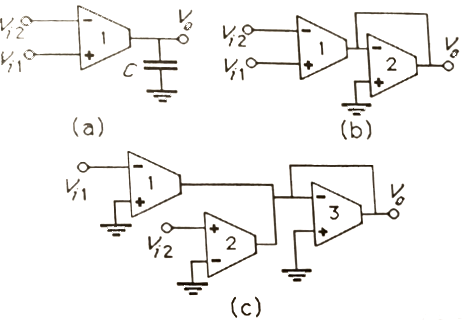
\includegraphics[scale=0.4]{otos.png}
\caption[Základní bloky s OTA]{Základní bloky s OTA a) integrující b) škálující c) sčítací \label{s:BLO}}
\end{figure}
\noindent Podle Schaumanna a Valkenburga \cite{13} blok a) na obrázku \ref{s:BLO} slouží k realizaci invertujícího nebo neinvertujícího integrátoru s~výsledným napětím
\begin{equation}
U_O = \frac{g_{m1}}{pC}(U_1 - U_2).
\end{equation}
Blok b) na obrázku \ref{s:BLO} je komparátor s různou polaritou a napětím na výstupu
\begin{equation}
U_O = \frac{g_{m1}}{g_{m2}}(U_1 - U_2).
\end{equation}
Blok c) na obrázku \ref{s:BLO} realizuje sčítací nebo rozdílový obvod s napětím na výstupu
\begin{equation}
U_O = -\frac{g_{m1}}{g_{m3}}U_1 + \frac{g_{m2}}{g_{m3}}U_2.\label{s:BLO3}
\end{equation}
\noindent Spojením těchto základních stavebních bloků se správnými znaménky lze získat různé funkční bloky.\\
Základním principem uplatňovaným při návrhu s OTA je použití pouze OTA a uzemněných kapacitorů, protože při návrhu IC jsou uzemněné kapacitory méně zatíženy parazitními chybami než plovoucí kapacitory. Pro IC použití je vhodné volit shodné transkonduktance. Parazitní vstupní a především výstupní impedance způsobují chyby ve výstupu filtru, což může vést na parazitní póly, které při vysokofrekvenčním použití nelze zanedbat. Při použití filtru pro zvukové aplikace (20--20\,000\,Hz) naopak lze chyby způsobené parazitními součástkami i~chyby způsobené konečnou šířkou pásma zanedbat, protože se jedná o nízký frekvenční rozsah.
\subsection{Odvození $\omega_0$, Q pro filtry 2. řádu}\label{s:ODV}
\noindent Náhradní obvod, ze kterého bude spočítána přenosová funkce pro přenos filtru druhého řádu, popisuje obrázek~\ref{s:DPO}.
\begin{figure}[h]
\centering
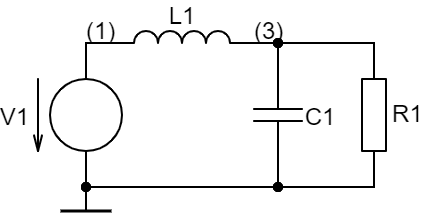
\includegraphics[scale=0.3]{circuit(1).png}
\caption{Dolní propust 2. řádu \label{s:DPO}} 
\end{figure}
\noindent Přenos obvodu byl vyjádřen jako
\begin{align}
H(p) = \frac{U_{out}}{U_{in}} = \frac{Z_2}{Z_1}, \quad Z_1 = pL + \frac{\frac{R}{pC}}{R + \frac{1}{pC}},\quad Z_2 = \frac{\frac{R}{pC}}{R + \frac{1}{pC}}.
\end{align}
Výsledný přenos je roven 
\begin{align}
H(p) = \frac{\frac{\frac{R}{pC}}{R + \frac{1}{pC}}}{pL + \frac{\frac{R}{pC}}{R + \frac{1}{pC}}}.
\end{align}
Elementárními algebraickými úpravami a následným vynásobením členem $1/(LRC)$ byl získán výsledný přenos.
\begin{align}\label{s:vzt4}
H(p) = \frac{R}{p^2LRC + pL + R} = \frac{\frac{1}{LC}}{p^2 + p\frac{1}{RC} + \frac{1}{LC}}.
\end{align}
\noindent Využitím poznatků ze sekce \ref{s:NAH} je možno za odpor a induktor dosadit do vztahu \ref{s:vzt4}.
\begin{align}
H(p) = \frac{\frac{1}{\frac{C_1C_2}{g_{m2}g_{m3}}}}{p^2 + p\frac{g_{m1}}{C_2} + \frac{1}{\frac{C_1C_2}{g_{m2}g_{m3}}}} = \frac{\frac{g_{m2}g_{m3}}{C_1C_2}}{p^2 + p\frac{g_{m1}}{C_2} + \frac{g_{m2}g_{m3}}{C_1C_2}}.
\end{align}
Porovnáním jmenovatele se jmenovatelem přenosu filtru 2. řádu byl obdržen vztah
\begin{align}
p^2 + p\frac{\omega _0}{Q} + \omega _0^2 &= p^2 + p\frac{g_{m1}}{C_2} + \frac{g_{m2}g_{m3}}{C_1C_2}.
\end{align}
Z tohoto vztahu byl vyjádřen mezní kmitočet jako 
\begin{align}
\omega _0^2 &= \frac{g_{m2}g_{m3}}{C_1C_2}, \\
\omega _0 &= \frac{\sqrt{g_{m2}g_{m3}C_1C_2}}{C_1C_2}
\end{align}
a činitel jakosti dosazením za $\omega _0$
\begin{align}
Q = \frac{\omega _0}{\frac{g_{m1}}{C_2}} = \frac{\sqrt{g_{m2}g_{m3}C_1C_2^3}}{C_1C_2g_{m1}}.
\end{align}
\subsubsection{Odvození $\omega_0$, Q pro obvod z obrázku \ref{s:V1}}
\begin{figure}[h]
\centering
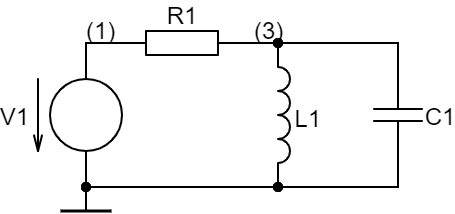
\includegraphics[scale=0.3]{rlc2(1).png}
\caption{Dolní propust 2. řádu (3 OTA) \label{s:RLC}} 
\end{figure}
\noindent Přenos obvodu na obrázku \ref{s:RLC} opět vyjádříme přes poměr výstupních a vstupních impedancí. 
\begin{align}
H(p) = \frac{U_{out}}{U_{in}} = \frac{Z_2}{Z_1}, \quad Z_1 = R + \frac{\frac{pL}{pC}}{\frac{1}{pC} + pL},\quad Z_2 = \frac{\frac{pL}{pC}}{\frac{1}{pC} + pL}
\end{align}
\begin{align}
H(p) &= \frac{\frac{\frac{L}{C}}{\frac{1 + p^2LC}{pC}}}{R + \frac{pLC}{C + p^2LC^2}} = \frac{\frac{pLC}{C + p^2LC^2}}{\frac{R(C + p^2LC^2) + pLC}{C + p^2LC^2}}\\
H(p) &= \frac{pLC}{RC + p^2RLC^2 + pLC} = \frac{pLC}{p^2 + p\frac{1}{RC} + \frac{1}{LC}}.
\end{align}
\noindent Dosazením za odpor a induktor ze sekce \ref{s:NAH} byl obdržen vztah
\begin{align}
H(p) = \frac{pC_2\frac{C_1}{g_{m2}g_{m3}}}{p^2 + p\frac{g_{m1}}{C_2} + \frac{1}{\frac{C_1C_2}{g_{m2}g_{m3}}}} = \frac{\frac{pC_1C_2}{g_{m2}g_{m3}}}{p^2 + p\frac{g_{m1}}{C_2} + \frac{1}{\frac{C_1C_2}{g_{m2}g_{m3}}}}.
\end{align}
Porovnáním jmenovatele se jmenovatelem přenosu filtru 2. řádu byl obdržen vztah
\begin{align}
p^2 + p\frac{\omega _0}{Q} + \omega _0^2 &= p^2 + p\frac{g_{m1}}{C_2} + \frac{g_{m2}g_{m3}}{C_1C_2}.
\end{align}
Z tohoto vztahu byl vyjádřen mezní kmitočet jako 
\begin{align}
\omega _0^2 &= \frac{g_{m2}g_{m3}}{C_1C_2}, \\
\omega _0 &= \frac{\sqrt{g_{m2}g_{m3}C_1C_2}}{C_1C_2}
\end{align}
a činitel jakosti dosazením za $\omega _0$
\begin{align}
Q = \frac{\omega _0}{\frac{g_{m1}}{C_2}} = \frac{\sqrt{g_{m2}g_{m3}C_1C_2^3}}{C_1C_2g_{m1}}.
\end{align}
Byly obdrženy identické vztahy jako v sekci \ref{s:ODV}.
\subsubsection{Odvození $\omega_0$, Q pro obvod z obrázku \ref{s:V2}}
\begin{figure}[h]
\centering
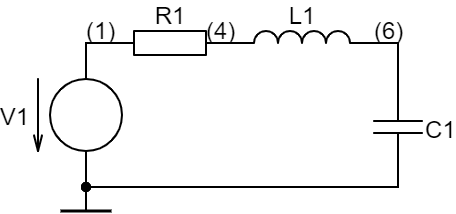
\includegraphics[scale=0.3]{Circuit(2).png}
\caption{Dolní propust 2. řádu (4 OTA) \label{s:RLC2}} 
\end{figure}
\noindent Přenos obvodu na obrázku \ref{s:RLC2} opět vyjádříme přes poměr výstupních a vstupních impedancí. 
\begin{align}
H(p) = \frac{U_{out}}{U_{in}} = \frac{Z_2}{Z_1}, \quad Z_1 = R + pL + \frac{1}{pC},\quad Z_2 = \frac{1}{pC}
\end{align}
\begin{align}
H(p) &= \frac{\frac{1}{pC}}{R + pL + \frac{1}{pC}} = \frac{1}{p^2LC + pCR + 1}.
\end{align}
\noindent Dosazením za odpor a induktor ze sekce \ref{s:NAH} byl obdržen vztah
\begin{align}
H(p) = \frac{1}{p^2\frac{C_1C_2}{g_{m3}g_{m2}} + p\frac{C_2}{g_{m1}} + 1} = \frac{g_{m1}g_{m2}g_{m3}}{p^2C_1C_2g_{m1} + pC_2g_{m2}g_{m3} + g_{m1}g_{m2}g_{m3}}
\end{align}
\noindent Elementárními algebraickými úpravami byl obdržen tvar
\begin{align}
H(p) = \frac{\frac{g_{m2}g_{m3}}{C_1C_2}}{p^2 + p\frac{g_{m2}g_{m3}}{C_1g_{m1}} + \frac{g_{m2}g_{m3}}{C_1C_2}}.
\end{align}
Porovnáním jmenovatele se jmenovatelem přenosu filtru 2. řádu byl obdržen vztah pro mezní kmitočet jako 
\begin{align}
\omega _0 &= \frac{\sqrt{g_{m2}g_{m3}C_1C_2}}{C_1C_2}
\end{align}
a činitel jakosti dosazením za $\omega _0$
\begin{align}
Q = \frac{\omega _0}{\frac{g_{m2}g_{m3}}{C_1g_{m1}}} = \frac{\sqrt{g_{m2}g_{m3}C_1^3C_2}g_{m1}}{C_1C_2g_{m2}g_{m3}}.
\end{align}